\subsection{Analytisches Haar-Wavelet}
\rhead{Analytisches Haar-Wavelet}
Betrachten wir zum Abschluss noch beispielhaft das Haar-Wavelet.
\begin{satz}
    Das zum reellen Haar-Wavelet analytische Wavelet ist
    \[\psi^\ast_{\text{Haar}} = \frac{1}{\sqrt{2}}\left(\psi_{\text{Haar}} + \frac{i}{\pi} \log\left|\frac{t^2-0.5^2)}{t^2}\right|\right).\]
\end{satz}

\begin{proof}
    Die Hilbert-Transformierte des Haar-Wavelets aus Definition~\ref{complex:def-haar} ist
    \begin{align*}
    \mathcal{H} \psi_{\text{Haar}}
    &= \frac{1}{\pi} \int_{-\infty}^{\infty} \frac{\psi_{\text{Haar}}(x)}{t-x} dx\\
    &= \frac{1}{\sqrt2\pi}\left( \int_{-0.5}^{0} \frac{1}{t-x}dx + \int_{0}^{0.5} \frac{-1}{t-x}dx \right)\\
    &= \frac{1}{\sqrt2\pi} \left( -\left[\log \left|t-x\right| \right]_{-0.5}^{0} + \left[\log\left|t-x\right| \right]_{0}^{0.5} \right)\\
    &= \frac{1}{\sqrt2\pi} \left( -\log\left|t\right| + \log\left|t+0.5\right| + \log\left|t-0.5\right| - \log\left|t\right|\right)\\
    &= \frac{1}{\sqrt2\pi} \log\left|\frac{(t+0.5)(t-0.5)}{t^2}\right|
    = \frac{1}{\sqrt2\pi} \log\left|\frac{t^2-0.5^2}{t^2}\right|.
    \end{align*}
    Das zugehörige, analytische Wavelet ist nach Satz~\eqref{complex:anawave}
    \[
    \psi^\ast_{\text{Haar}} = \frac{1}{\sqrt{2}}\left(\psi_{\text{Haar}} + \frac{i}{\pi} \log\left|\frac{t^2-0.5^2)}{t^2}\right|\right).\qedhere
    \]
\end{proof}

Das analytische Haar-Wavelet ist in Abbildung~\ref{complex:haar} dargestellt.
Es hat keinen kompakten Träger mehr.
Gut ersichtlich ist dafür die Symmetrie, der Realteil ist eine ungerade Funktion, folglich ist der Imaginärteil gerade.
Die graue Fläche zeigt deutet den Betrag der Funktion an.
Bei analytischen Wavelets ist der Betrag gleich der Envelope.
Die Energie des analysierten Signals geht also immer entweder in den Real- oder Imaginärteil der Analyse, was sich wieder in der gewünschten Eigenschaft zeigt, Amplitude und Phase unabhängig betrachten zu können.

\begin{figure}
	\centering
	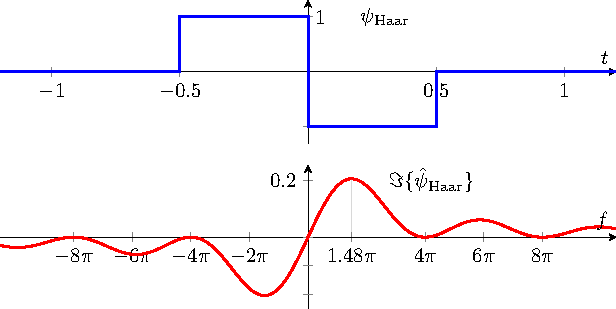
\includegraphics{papers/complex/images/haar.pdf}
	\caption{Das analytische Haar-Wavelet, Realteil in Blau und Imaginärteil in Rot. \label{complex:haar}}
\end{figure}